\chapter{Application: Strong Edge Colouring}
\label{chap:strong_edge_colouring}

As defined in the \hyperref[sec:intro_strong_edge_coloring]{introduction}
a strong edge colouring of a graph is an edge colouring where two edges which are incident to some
common edge must have different colours.

We can view a strong edge colouring of a graph as a proper vertex colour of $L(G)^2$, the
square of the line graph of $G$ \cite{molloyBoundStrongChromatic1997}.
The line graph $L(G)$ is a graph with a vertex $v_e$ for
each $e\in E(G)$ such that $\{v_e, v_f\} \in E(L(G))$ iff $e$ is incident to $f$ in
$G$. The square of a graph $G^2$ then is a copy of the graph where vertices at distance $\leq 2$
are connected. See figure \ref{fig:lg_example} for an example construction.

\begin{figure}[ht]
    \centering
    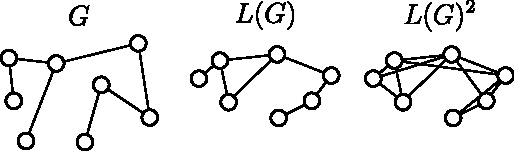
\includegraphics{LG_example}
    \caption{Example $G$, $L(G)$ and $L(G)^2$}
    \label{fig:lg_example}
\end{figure}

\begin{definition}[Strong Neighbourhood]
    Given a graph $G$ and edge $E \in E(G)$ define the strong neighbourhood
    $N_s(e)$ of $e$ as those edges $f \in E(G)$ which are adjacent to $e$ in 
    $L(G)^2$ (i.e. those which cannot share a colour with $e$ in a strong edge colouring).
\end{definition}

\section{The Erd\H{o}s and Nešetřil conjecture}

Erd\H{o}s and Nešetřil \cite{faudreeInducedMatchingsBipartite1989} conjectured an
upper bound on the strong chromatic index $\chi'_s(G)$, the minimum colours needed for
a strong edge colouring.

\begin{conjecture}[Erd\H{o}s, Nešetřil 1989 \cite{faudreeInducedMatchingsBipartite1989}]
    \[\chi'_s(G) \leq 1.25\Delta(G)^2.\]
\end{conjecture}

The bound of $2\Delta(G)^2$ was the best known bound until 1997 when Molloy and Reed
showed the following.
\begin{knowntheorem}[Molloy, Reed 1997 \cite{molloyBoundStrongChromatic1997}]
    If $\Delta(G)$ is sufficiently large then
    $\chi'_s(G) \leq 1.998\Delta(G)^2$.
\end{knowntheorem}

Their proof consisted of colouring $L(G)^2$ with 2 discrete steps:
The first is a bound on the edge density of any neighbourhood of $L(G)^2$. We call
this the \textit{strong neighbourhood density}.
\begin{knownlemma}[Lemma 1 from \cite{molloyBoundStrongChromatic1997}]
    If $G$ has maximum degree $\Delta$ then for each $e\in E(G)$
    $|N_s(e)| \leq (1-\frac{1}{36})\binom{2\Delta^2}{2}$.
\end{knownlemma}
After showing the strong neighbourhoods in $L(G)^2$ are sparse they use a colouring
lemma to colour $L(G)^2$:
\begin{knownlemma}[Lemma 2 from \cite{molloyBoundStrongChromatic1997}]
    Let $\delta, \gamma > 0$ satisfy some condition. Then if
    $\Delta(H) \leq X$ such that $N(v)$ has at most $(1-\delta)\binom{X}{2}$ edges
    then $\chi(H)\leq (1-\gamma)X$.
\end{knownlemma}

This strategy of bounding the edge density of strong neighbourhoods of $G$ and
using a probabilistic colouring was iterated on through successive papers:
Bruhn and Joos found an asymptotically tight bound on the strong neighbourhood density
and improved the colouring lemma.
\begin{knowntheorem}[Bruhn \& Joos, 2015 \cite{bruhnStrongerBoundStrong2018}]
    If $\Delta(G)$ is sufficiently large then
    $\chi'_s(G) \leq 1.93\Delta(G)^2$.
\end{knowntheorem}
Bonamy, Perett and Postle introduced a modification of the method where rather than
bounding the strong edge neighbourhood density for the entire graph we instead focus
on a subgraph of $L(G)^2$ of high degree vertices. They show that the
neighbourhood density in this subgraph can go below the tight bound of Bruhn and Joos
and so can be coloured with fewer colours. The rest of the graph has low degree so can
be coloured greedily.

\begin{knowntheorem}[Bonamy, Perrett \& Postle, 2018 \cite{bonamyColouringGraphsSparse2018}]
    If $\Delta(G)$ is sufficiently large then
    $\chi'_s(G) \leq 1.835\Delta(G)^2$.
\end{knowntheorem}

Most recently then Hurley, de Verclos and Kang improved on the colouring lemma from the
Bonamy et al. paper to achieve the current lowest known bound.
\begin{knowntheorem}[Hurley, de Verclos \& Kang, 2022 \cite{hurleyImprovedProcedureColouring2022}]
    If $\Delta(G)$ is sufficiently large then
    $\chi'_s(G) \leq 1.772\Delta(G)^2$.
\end{knowntheorem}

In this chapter we use the semidefinite method on local flags to improve the strong
neighbourhood density bound, then applying the colouring lemma from Hurley et al. as a black
box we claim the following result.

\begin{theorem}
    If $\Delta(G)$ is sufficiently large then $\chi'_s(G) \leq 1.73\Delta(G)^2$.
\end{theorem}

\section{Reduction}

The theorem that we want to improve on is the strong edge neighbourhood theorem from
the Bonamy et al. paper which appears in Hurley et al. as follows:
\begin{knowntheorem}[Theorem 3.1 \cite{hurleyImprovedProcedureColouring2022}]
    Fix $\eta \in [0, 0.3]$. For any graph $G$ let $H=L(G)^2$. Let $F$ be a
    maximum subset of $V(H)$ such that $H[F]$ has minimum degree
    $\geq (2-\eta)\Delta(G)^2$. Then for any $f\in F$ the number of edges in the subgraph
    $H[N_{H[F]}(f)]$ induced by the neighbourhood of $f$ (in $H[F]$) is at most
    \[
        \left(\frac{31}{6} - \frac{128}{10-3\eta} - \eta^2\right)\Delta(G)^4
    \]
\end{knowntheorem}

In other words we are given a graph $G$ and a maximal subset of the edges $F \subseteq E(G)$
such that the subgraph induced by $F$ in $H=L(G)^2$ has minimum degree
$\geq (2-\eta)\Delta(G)^2$ for some $\eta$. This means each $f \in F$ has
at least $(2-\eta)\Delta(G)^2$ other edges $f' \in F$ adjacent in $L(G)^2$
($|N_s(f) \cap F| \geq (2-\eta)\Delta(G)^2\ \forall\ f \in F$).
We can then just consider the graph $H[F]$ induced by this high degree $F$ subset.
Then for some fixed $f \in F$ we want to find an upper bound on the number of edges
in its neighbourhood in $H[F]$. That is, the number of pairs $e, e' \in N_s(f) \cap F$ such
that $e, e'$ adjacent in $L(G)^2$.

As we did in section \ref{sec:counting_pentagons} we want to reduce this to a problem
on coloured graphs.
Given $G$, $F\subseteq E(H)$, $\eta > 0$ and $f \in F$ as above we can construct a
new corresponding $(2,2)$-graph (red/black vertices, red/black edges) $G'$ as follows:
Let $f=\{u, v\}$. Take a copy of $G$ and colour all neighbours of $u$ and $v$ black
and all other vertices red. Then colour every edge $e \in F$ black and all other
edges red.

\begin{lemma}
    Let $G, F, \eta, f$ and $G'$ be as above then the number of edges in $H[N_{H[F]}(f)]$
    where $H=L(G)^2$ is equal to the number of pairs of black edges in $G'$
    which have a common incident edge and at least one of the vertices of each
    edge is black plus some $o(\Delta(G)^4)$ term.
\end{lemma}

\begin{proof}
    Let $G, F, \eta, f$ and $G'$ be as above. Consider some edge $\{e, e'\}$ in
    $H[N_{H[F]}(f)]$. Both of these $e,e'$ are in $F$ so is coloured black in $G'$.
    Similarly both are in the strong neighbourhood of $F$ meaning each has a common
    incident edge with $f$. Edges incident to $f$ have both vertices coloured black
    in $G'$ so each of $e, e'$ has at least one black vertex.
    Hence this edge $\{e, e'\}$ corresponds to a pair of black edges with at least one
    black vertex each in $G'$ at distance $\leq 2$ from each other.

    Consider then some pair $e,e' \in E(G')$ where both are black edges
    and have at least one black vertex and are at distance $\leq 2$ from each other.

    As each has a black vertex they must be either incident to $f$ \textit{or} equal
    to $f$. If both $e, e' \neq f$ then
    $e, e'$ satisfy exactly the conditions to be an edge in $H[N_{H[F]}(f)]$.
    Hence we overcount the number of edges in $H[N_{H[F]}(f)]$ by exactly the
    number of these pairs $e, e'$ where one of $e, e' = f$. Assume $e=f$,
    this leaves only $\leq 2\Delta(G)^2$ choices for $e'$ so there are at most
    $2\Delta(G)^2$ such pairs which is $o(\Delta(G)^4)$ as required.
\end{proof}
